\begin{tabular}{ccc}
    \begin{tikzpicture}
    \node[circle,radius=1cm,draw,thick] (x) at (0,0) {$\times$};
    \node[above=1.5cm] (deltatrain) at (x) {$p(t) = \sum_{n=-\infty}^{\infty} \delta(t-n(T+\Delta))$};
    \node[left=1.5cm] (x_t) at (x) {$x(t)$} ;
    \node[right=1.5cm,rectangle,draw,thick,inner sep=0.5cm] (H_jw) at (x) {$H(j\omega)$} ;
    \node[right=2cm] (x_r) at (H_jw) {$y(t)$} ;
    \node[above=5cm,right=.4cm] at (x.north) {$x_p(t)$} ;
    
    \draw[->,very thick] (deltatrain) -- (x) ;
    \draw[->,very thick] (x_t) -- (x) ;
    \draw[->,very thick] (x) -- (H_jw) ;
    \draw[->,very thick] (H_jw) -- (x_r) ;
    \end{tikzpicture} & \hfill &
    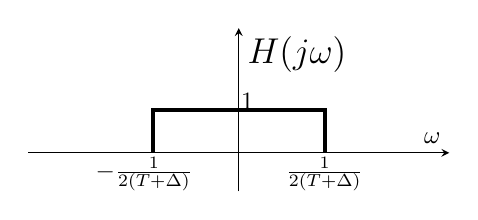
\begin{tikzpicture}[scale=0.9,transform shape]
    \begin{axis}[
        x=0.05\textwidth,y=0.05\textwidth,
        axis y line=center,
        axis x line=middle,
        xlabel=$\omega$,ylabel={\Large $H(j\omega)$},
        xmin=-4.9,xmax=4.9,
        ymin=-0.9,ymax=2.9,
        ticks=none
        ]
        \addplot[
        black,
        ultra thick
        ] coordinates {
            (-2,0) (-2,1) (2,1) (2,0)
        } ;
        \node at (-2.2,-.5) {$-\frac{1}{2(T+\Delta)}$};
        \node at (2,-.5) {$\frac{1}{2(T+\Delta)}$};
        \node at (0.2,1.2) {1} ;
    \end{axis}
    \end{tikzpicture}
    \end{tabular}